%
% firmware.tex
%
% Copyright (C) 2020 by Universidade Federal de Santa Catarina.
%
% OBDH 2.0 Documentation
%
% This work is licensed under the Creative Commons Attribution-ShareAlike 4.0
% International License. To view a copy of this license,
% visit http://creativecommons.org/licenses/by-sa/4.0/.
%

%
% \brief Firmware chapter.
%
% \author Gabriel Mariano Marcelino <gabriel.mm8@gmail.com>
%
% \institution Universidade Federal de Santa Catarina (UFSC)
%
% \version 0.1.0
%
% \date 30/10/2019
%

\chapter{Firmware} \label{ch:firmware}

\section{Tasks}

A list of the firmware tasks can be seen in the \autoref{tab:firmware-tasks}.

\begin{table}[!h]
    \centering
    \begin{tabular}{llllll}
        \toprule[1.5pt]
        \textit{Name}          & \textit{Priority} & \textit{Initial delay [ms]} & \textit{Period [ms]} & \textit{Stack [bytes]} \\
        \midrule
        Startup (boot)         & Highest           & 0                           & Aperiodic            & 500                    \\
        Deployment hibernation & Highest           & 0                           & Aperiodic            & TBD                    \\
        Antenna deployment     & Highest           & 0                           & Aperiodic            & TBD                    \\
        Watchdog reset         & Lowest            & 0                           & 100                  & TBD                    \\
        Heartbeat              & Lowest            & 0                           & 500                  & 128                    \\
        Periodic downlink      & Medium            & 5000                        & 60000                & 128                    \\
        Uplink                 & High              & 5000                        & 1000                 & TBD                    \\
        EPS reading            & Medium            & 5000                        & 60000                & TBD                    \\
        EDC reading            & High              & 5000                        & 1000                 & TBD                    \\
        Payload X reading      & Medium            & 5000                        & 5000                 & TBD                    \\
        TTC writing            & Medium            & 5000                        & 10000                & TBD                    \\
        Radio periodoc reset   & Low               & 0                           & 600000               & TBD                    \\
        System reset           & High              & 0                           & 36000000             & 128                    \\
        Read temperature       & Low               & 0                           & 60000                & TBD                    \\
        \bottomrule[1.5pt]
    \end{tabular}
    \caption{Firmware tasks.}
    \label{tab:firmware-tasks}
\end{table}

All these tasks are better described below.

\subsection{Startup (boot)}

.

\subsection{Deployment hibernation}

.

\subsection{Antenna deployment}

.

\subsection{Watchdog reset}

This task resets the internal and external watchdog timer at every 100 ms. The internal watchdog has a maximum count time of 500 ms, and the external watchdog a maximum of 1600 ms (see \autoref{ch:hardware} for more information about the watchdog timers).

To prevent the system to not reset during an anomaly on some task (like an execution time longer than planned), this task has lowest possible priority: 0.

\subsection{Heartbeat}

The heartbeat task keeps blinking a LED (``\textit{System LED}'' in \autoref{fig:status-leds}) at a rate of 1 Hz during the execution of the system. Its purpose is to give a visual feedback of the execution of the scheduler. This is tasks does not have a specific purpose on the flight version of the module (the flight version of the PCB does not have LEDs).

\subsection{Periodic downlink}

.

\subsection{Uplink}

.

\subsection{EPS reading}

.

\subsection{EDC reading}

.

\subsection{Payload X reading}

.

\subsection{TTC writing}

.

\subsection{Radio periodic reset}

.

\subsection{System reset}

This task resets the microcontroller by software at every 10 hours. This can be useful to cleanup possible wrong values in variables, repeat the antenna deployment routine (limited to $n$ times), cleanup the RAM memory, etc.

\subsection{Read temperature}

This task reads the internal temperature of the microcontroller of the OBDH at every 60 seconds.

\section{Telecommands}

\begin{table}[!h]
    \centering
    \begin{tabular}{lll}
        \toprule[1.5pt]
        \textit{Name}          & \textit{Parameters}           & \textit{Access} \\
        \midrule
        Enter hibernation      & Hibernation period in seconds & Private         \\
        Leave hibernation      & None                          & Private         \\
        Activate beacon        & None                          & Private         \\
        Deactivate beacon      & None                          & Private         \\
        Activate downlink      & None                          & Private         \\
        Deactivate downlink    & None                          & Private         \\
        Activate EDC           & None                          & Private         \\
        Deactivate EDC         & None                          & Private         \\
        Get EDC info           & None                          & Private         \\
        Activate Payload X     & Experiment period in seconds  & Private         \\
        Deactivate Payload X   & None                          & Private         \\
        Set system time        & Time value (epoch)            & Private         \\
        Ping                   & None                          & Public          \\
        Message broadcast      & ASCII message                 & Public          \\
        Request data           & Data flags                    & Public          \\
        \bottomrule[1.5pt]
    \end{tabular}
    \caption{System telecomamnds.}
    \label{tab:system-telecommands}
\end{table}

\subsection{Enter hibernation}

.

\subsection{Leave hibernation}

.

\subsection{Activate beacon}

.

\subsection{Deactivate beacon}

.

\subsection{Activate EDC}

.

\subsection{Deactivate EDC}

.

\subsection{Get EDC info}

This telecommand request information from the EDC payload. When received, the OBDH transmits the housekeeping and state frames of the EDC module (28 bytes). This telecommand does not requires a key.

\subsection{Activate Payload X}

.

\subsection{Deactivate Payload X}

.

\subsection{Set system time}

.

\subsection{Ping}

.

\subsection{Message broadcast}

.

\subsection{Request data}

.

\section{Operating System}

FreeRTOS 10

\section{Hardware Abstraction Layer (HAL)}

DriverLib

\section{Protocols}

\subsection{NGHam}

NGHam \cite{ngham}, short for Next Generation Ham Radio, is a set of protocols for packet radio communication. Its usage is similar to the existing AX.25 protocol.

\begin{figure}[!ht]
    \begin{center}
        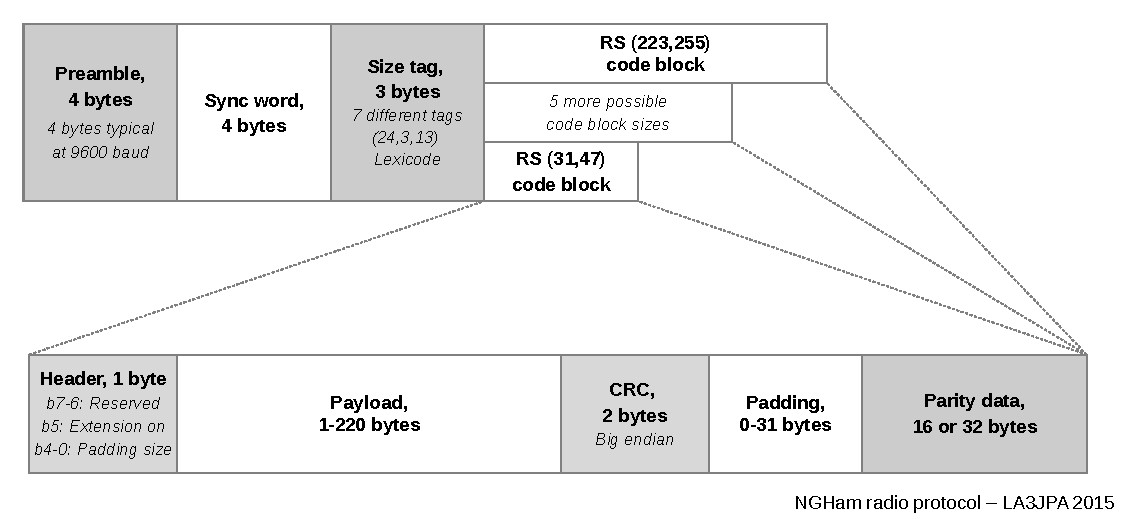
\includegraphics[width=\textwidth]{figures/ngham_block_v4.pdf}
        \caption{NGHam packet structure.}
        \label{fig:ngham-stack}
    \end{center}
\end{figure}
